\documentclass{standalone}
\usepackage{tikz}
\usepackage{ctex,siunitx,ninecolors}
\setCJKmainfont{Noto Serif CJK SC}
\usepackage{tkz-euclide}
\usepackage{amsmath}
\usepackage{wasysym}
\usetikzlibrary{patterns, calc}
\usetikzlibrary {decorations.pathmorphing, decorations.pathreplacing, decorations.shapes,}
\begin{document}
\small
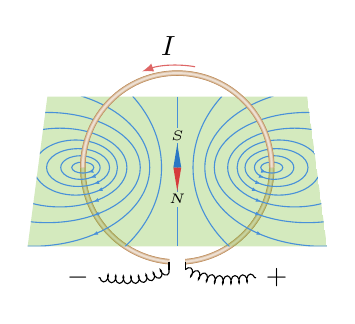
\begin{tikzpicture}[>=latex,scale=1]
  \foreach \x in {80,60,40,20}
  {
    \draw[line width={2*sin(\x)},brown5!\x](-1.2,0)arc(180:265:1.2);
    \draw[line width={2*sin(\x)},brown5!\x](1.2,0)arc(0:-85:1.2);
  }
  \begin{scope}
    \clip (1.9,-1)--(1.65,0.9)--(-1.65,0.9)--(-1.9,-1);
    \path [fill=olive7,opacity=0.3](1.9,-1)--(1.65,0.9)--(-1.65,0.9)--(-1.9,-1);
    \draw[azure6](0,0.9)--(0,-1);
    \fill[azure5](-0.05,0)--(0,0.3)node[above,fill=olive7!30,text=black,inner sep=1pt]{\tiny $S$}--(0.05,0);
    \fill[red5](-0.05,0)--(0,-0.3)node[below,fill=olive7!30,text=black,inner sep=1pt]{\tiny $N$}--(0.05,0);
    \foreach \x/\ra/\rb in {1.2/0.14/0.07,1.23/0.25/0.15,1.26/0.4/0.24,1.29/0.53/0.35,1.49/0.85/0.5,1.65/1.18/0.7,1.85/1.5/1.0,2.15/1.95/1.55}
    {
      \draw[azure6, postaction={decorate},decoration={markings,mark={at position 0.65 with {\arrow{Latex[scale=0.4]}}}}](\x,0)ellipse[x radius=\ra cm, y radius=\rb cm];
      \draw[azure6, postaction={decorate},decoration={markings,mark={at position 0.85 with {\arrowreversed{Latex[scale=0.4]}}}}](-\x,0)ellipse[x radius=\ra cm, y radius=\rb cm];
    }
  \end{scope}
  \foreach \x in {80,60,40,20}
  {
    \draw[line width={2*sin(\x)},brown5!\x](-1.2,0)arc(180:0:1.2);
  }
  \draw[->,red6](80:1.3)arc(80:110:1.3)node[midway,above,text=black]{$I$};
  \draw(265:1.2)--++(-0,-0.1)(-85:1.2)--++(-0,-0.1);
  \draw[decorate,decoration={coil,segment length=1mm,amplitude=0.5mm}]([yshift=-1mm]265:1.2)..controls(-0.5,-1.5)and(-0.8,-1.4)..(-1,-1.4)node[left]{$-$};
  \draw[decorate,decoration={coil,segment length=1mm,amplitude=0.5mm}]([yshift=-1mm]-85:1.2)..controls(0.5,-1.5)and(0.8,-1.4)..(1,-1.4)node[right]{$+$};
\end{tikzpicture}
\end{document}